\documentclass[journal]{IEEEtran}
\usepackage[utf8]{inputenc}
\usepackage{lipsum}
\usepackage{graphicx}
\usepackage[colorinlistoftodos, ]{todonotes}


\title{Ericsson HB107\\\Large{The first smartphone platform with high quality camera}}
%\author{C.~Aknesil, J.~Altayó}
\author{Michael~Shell,~\IEEEmembership{Member,~IEEE,
} John~Doe,~\IEEEmembership{Fellow,~OSA,} and~Jane~D
oe,~\IEEEmembership{Life~Fellow,~IEEE}%
\thanks{Manuscript received January 20, 2002; revise
d August 26, 2015. This work was supported by the IE
EE.}%
\thanks{M. Shell was with the Georgia Institute of T
echnology.}}

\date{September 2019}

\begin{document}
\maketitle

\todo{CORRECT THE AUTHORS}

\begin{abstract}
The authors conducted an interview with Mr.~Tobias~Lindquist, an Ericsson employee, and project manager. 
The focus was put on the HB107 project, with the main objective as the development and maintenance of a smartphone platform of the Sony Ericsson line. Several aspects of the project are discussed. The main goals was to finish the project on time. The organization of the project had a deep hierarchy consisting of more than four layers of sub-projects. The traditional project management is applied to at least top two layers of the project. Agile methodologies are sometimes applied to sub-projects of more than three layers. The management team had to deal with a long list of risks, delays in mass production being the one related to the worst consequence.
\end{abstract}

\begin{IEEEkeywords}
    Project Management, Interview, PROPS, Smartphones
\end{IEEEkeywords}

\section{Introduction}
The authors conducted an interview with Mr.~Tobias~Lindquist, an Ericsson employee, and project manager. During this interview, several aspects of the project manager position were discussed as well as particular details of a previous project named HB107, including the methods, organization, and outcomes of this project. 

This assignment aims to help the authors obtain a better understanding of what a project manager tasks consist of. By interviewing an active project manager, a different point of view is obtained as opposed to only relying on the theoretical lectures given during the course.

\section{The Project}
During the interview, the focus was put on the HB107 project. This project was initiated in 2007 and its main objective was the development and maintenance of a smartphone of the Sony Ericsson line for three years.

\subsection{Goals and Directives}
The main goal of the project was to complete the development of the smartphone platform in a very limited amount of time. 

\begin{figure}[h]
    \centering
    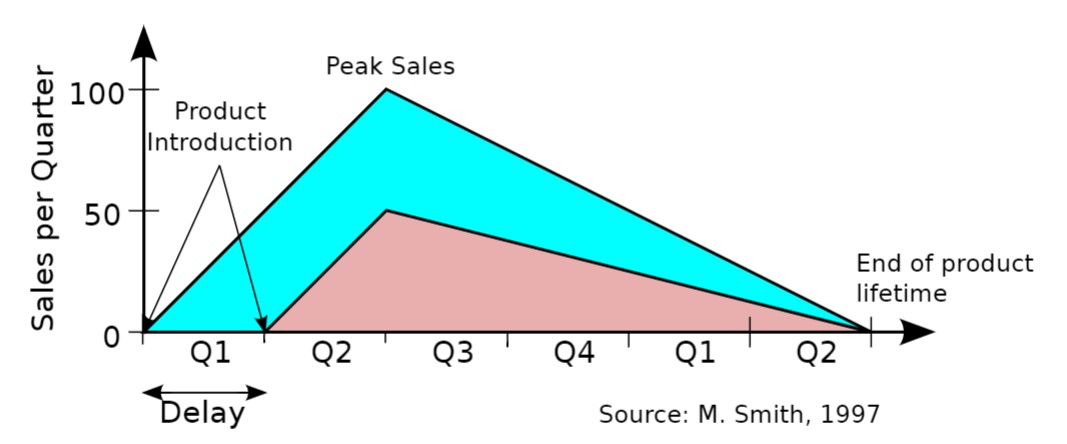
\includegraphics[width=\linewidth]{sales.jpg}
    \caption{Comparison of sales for different product introduction times}
    \label{fig:sales}
\end{figure}

As can be seen in Fig.~\ref{fig:sales} the total amount of sales (the area underneath the lines) varies significantly if the product is introduced with a delay. This is especially true for the case of smartphones and more intense during the late 2000s. This is the main reason why the most important goal of the project was to be able to release the product in a short time.

The second major directive given was to achieve a successful amount of features introduced in the new generation of smartphones. This was decided in conjunction with the technical managers and the market analysts at the beginning of the project. Although a basic set of requirements was fixed, modifications or additions to that set could be introduced due to several reasons, for example, a competitor introducing a feature and forcing the other companies to match that feature if they want to stay competitive.

Finally, the last major target was keeping the cost per unit (the money one should pay to buy one mobile phone) as low as possible. 

\section{The Challenges}
A project of big magnitude such as this one involves many challenges that needs to be adressed during the development and management strategies.
\subsection{The Time Constraint}
The biggest challenge was the time constraint. 

During the late 2000s, the competition among several smartphone manufacturers was of monumental dimensions, even greater than today since the technological gap between smartphone generations was much bigger in the 2000s than in the present times. This imposed several challenges, hard deadlines being the biggest one, on the project. Not being able to deploy the product in time meant not being able to offer the state of the art technology to the customers. This presented the risk of the product being obsoleted by better products released by competitive companies.

\subsection{Complex Requirement Analysis}
The second biggest challenge was performing the requirement analysis and defining the scope of the platform under development. This challenge became even more complicated combined with the time constraint. The reason that makes this task complex is the existence of contradictory objectives. One objective is that the platform should be designed in a configurable and expendable way so that it can accommodate multiple versions of the product, at the same time will facilitate the development of future generations. However, a very high volume of production and predicted sales required the design decision is made as early as possible.

Another importance of the requirement analysis is that at the end of the analysis, what to produce by the factories will be decided. Figuring our mass production requirements is very important since the biggest part of the budget is spent on production, not the development. Moreover, because of the very high volume, starting the production as early as possible is crucial. 

\subsection{Technical Difficulties}
The third biggest challenge is the technical difficulties behind developing a mobile platform. This process is very difficult because of the scope and diversity of interconnected sub-tasks. As opposed to today, during 2000s companies had to develop the mobile phones from the head to toe including design, implementation, verification, and production of ASIC chips, analog and digital circuits, software, which can be divided as firmware, operating system, drivers, applications, GUI, etc. Being capable of finalizing such a project in limited time required advanced project and risk management. 

\section{The Organization}
The organization of the project was very complex, given the requirements and challenges mentioned above, and related to this involvement of thousands of participants in the project, including engineers, sales agents, market analysts, and management staff. 

\begin{figure}[h]
    \centering
    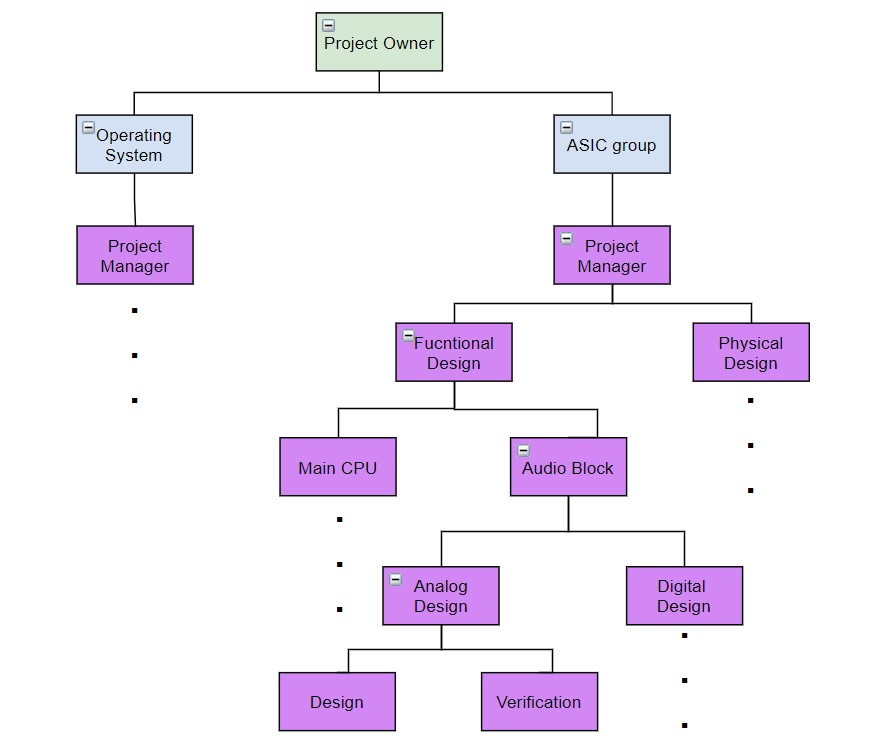
\includegraphics[width=\linewidth]{project_structure.jpg}
    \caption{Example of the Project Structure}
    \label{fig:project_structure}
\end{figure}

\subsection{Internal Structure}
The project was divided into more than three levels of sub-projects. The main project was managed by a team of high managers including Mr.~Lindquist. Each sub-project had separate managers, project managers, technical team leaders. For some complex projects, like the main processing ASIC, the sub-divisions could continue for up five nested sub-projects. An explanatory diagram can be seen in Fig.~\ref{fig:project_structure}. It should be noted that this is an example based on the explanations given by Mr.~Tobias since the real structure division is not public.

This complex organization imposed several challenges, one of them being the difficulty of parallelizing the work among different sub-projects. Fortunately, the system architecture was not experiencing big changes (explained later in more detail), so projects had fixed interfaces among them from the beginning of the project.

\subsection{Internal Comunicacion}
Communication was essential to achieve progress in interconnected sub-projects performed by different teams, the teams developing part of the hardware that has a common interface for instance. Project managers made sure the teams had the means to communicate.  

\todo{Elaborate, how did they enable communication?}

\section{The Methodology}
A traditional management approach was used for higher levels of management. The time required from the beginning of the project to the release of the first version was very long, about one year. Together with time-to-market constraints and high competition prevented the use of agile project management. There was no resource to support agile development in the higher levels because of long-term commitments: factories had to be prepared, employees had to be trained, etc. 

The project was planned in detail beforehand, had clear milestones and tollgates, and it was made sure it was developed and verified sufficiently before the first release. Making updates on products was not possible, as opposed to today. These facts made mobile platform development "one-shot" projects. Contracts with other companies, such as telecom operators, require fixed deadlines and features/requirements for the finished product, rather than flexible specifications. Customers wanted a high commitment to the deadline.

The majority of projects that are developed by Ericsson, including HB107, used a PROPS-based management method, which is developed by Ericsson during the late '80s to be used internally. One modification to the PROPS methodology was the introduction of multi-line organizations. For example, the R\&D department had an independent budget from the rest. Furthermore, the company was running more than one overlapping projects. So handling of multiple independent budgets and allocation of them to more than one simultaneous project should have been handled by the project methodology. 

Trial and error cycles were between projects rather than during the project.

However, sub-project management was independent. Starting from the second level sub-projects, especially in software development, agile was possible and used extensively.



Furthermore, A great variety of IT tools was used to achieve successful communication among the development teams and management committees, spreadsheet documents being the most popular one. Most of them consisted of web-based checklists that each individual was asked to fill frequently.

\section{The Implementation}
The key focus during the project management was put on active project management. Instead of relying on deadlines or tollgates, performance indicators were continuously analyzed to allow the management team to anticipate possible issues during the development. 

One of the methods to achieve this to monitor the communication between team members and teams. Occurrences of problems and discussions is a good sign, lack of communication is an indication that something is going wrong. 

A similar method is to monitor the verification process: if predicted errors do not reveal themselves, this means the verification process is insufficient. 

\begin{figure}[h]
    \centering
    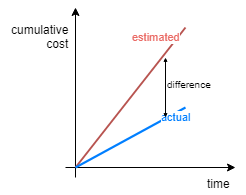
\includegraphics[width=0.8\linewidth]{cost.png}
    \caption{Cumulative cost of the project}
    \label{fig:cost}
\end{figure}

A very good example that Mr.~Tobias provided was to look at the cumulative cost of the project. As can be seen in Fig.~\ref{fig:cost}, the cumulative cost of a project can be estimated at the beginning of such. During the development the management committee can pay attention to the actual cumulative cost and observe is a substantial difference exists. This method is significantly better than relying on milestones and tollgates since it can anticipate problems during the development so correction measurements can be taken before it is too late.

An interesting comment from Mr.~Tobias in the interview was that workers will tend not to communicate issues at an early stage since they will be confident that the issue can be solved by themselves. On many occasions, this can generate major delays if a different method was used.

\section{The Risk Management \& The Risks}
The HB107 project had to deal with a long list of risks and uncertainties that were discussed during the interview. Even though smartphone development was not a new industry, unexpected problems were common, as explained below, and consequences of these problems were magnified by the time constraint. 

\subsection{The Risk Management}
The management of risks were performed starting from the requirement analysis, however this management was very difficult since competition with other companies forced some of the risks to be taken. In case of an unexpected problem, every possible resource, including the ones allocated to other projects, was temporarily redirected to solve the pop-up problem.

\subsection{The Risks}
One of the biggest issues that could occur during the mass production was the suppliers not being able to deliver the amounts of components required to produce the devices. This event could break the supply chain and generate a lack of stocks that could have a negative impact on the sales of the product.

Another potential problem was the possibility of a specific component unexpectedly not meeting the quality requirements. Mr.~Tobias mentioned a situation (not related to this project) where a metallic piece of a smartphone was getting corroded during a weather test where the device where introduced in a damp environment. These king of issues can force a redesign around that component. Fortunately, it was in an early stage of prototyping and there was not a major impact on the overall project.

Issues or malfunctions found during beta-testing were also a major concern during the project. Mr.~Tobias mentioned a case where the battery of a smartphone cached fire during a test. Fortunately, the test user was not harmed but a major redesigned had to be done to ensure a safe product when this was released to the main public.

\section*{Acknowledgments}
The authors would like to thank both  Mr.~Tobias~Lindquist and Mr.~Thomas Magnusson for helping us to conduct the interview for this course.
\end{document}
